\documentclass[sigconf,nonacm]{acmart}
\settopmatter{printacmref=false,printfolios=true}
\setcopyright{none}
\renewcommand\footnotetextcopyrightpermission[1]{}
\usepackage{amsmath,tabularx,array,enumitem,balance}
\definecolor{CourseBlue}{HTML}{315EFB}
\definecolor{CourseTeal}{HTML}{14877D}
\hypersetup{colorlinks=true,linkcolor=CourseBlue,citecolor=CourseTeal,urlcolor=CourseTeal}
\newcolumntype{Y}{>{\raggedright\arraybackslash}X}
\setlist{leftmargin=*,topsep=3pt,itemsep=2pt}
\newcommand{\CourseNumber}{COMSCI/ECON 206}
\newcommand{\CourseName}{Computational Microeconomics}
\newcommand{\CourseSession}{Autumn 2026 Session 1}
\newcommand{\Instructor}{Luyao Zhang}
\newcommand{\WorkshopSession}{Session E}
\newcommand{\GitHubLink}{\url{https://github.com/cccc-0212/yichen-ps1-overleaf} (code commit: \texttt{205d90528691b0497aca09525c69dc9e3f289d73})}
\newcommand{\TemplateRepository}{\url{https://github.com/sunshineluyao/ps1-overleaf-template}}
\newcommand{\ColabLink}{\url{https://colab.research.google.com/github/cccc-0212/yichen-ps1-overleaf/blob/yichen_proposal/companion/notebooks/adaptive_tax_game.ipynb}}
\newcommand{\DemoLink}{\url{https://huggingface.co/spaces/dku-comsci-econ206-2026/yichenshendemo}}
\newcommand{\coursemeta}{\noindent\textbf{Submission to:} \CourseNumber{} --- \CourseName.\\
\textbf{Course session:} \CourseSession. \textbf{Workshop:} \WorkshopSession.\\
\textbf{Instructor:} \Instructor. \textbf{Assignment:} PS1 research proposal.\par\smallskip}
\title{Transparent Adaptive Taxation under Limited Information: A Repeated-Game Stress Test}
\author{Yichen Shen}
\affiliation{\institution{Duke Kunshan University}\city{Kunshan}\country{China}}
\email{ys479@duke.edu}
\renewcommand{\shortauthors}{Shen}

\begin{document}
\begin{teaserfigure}
\captionsetup{skip=8pt}
\centering
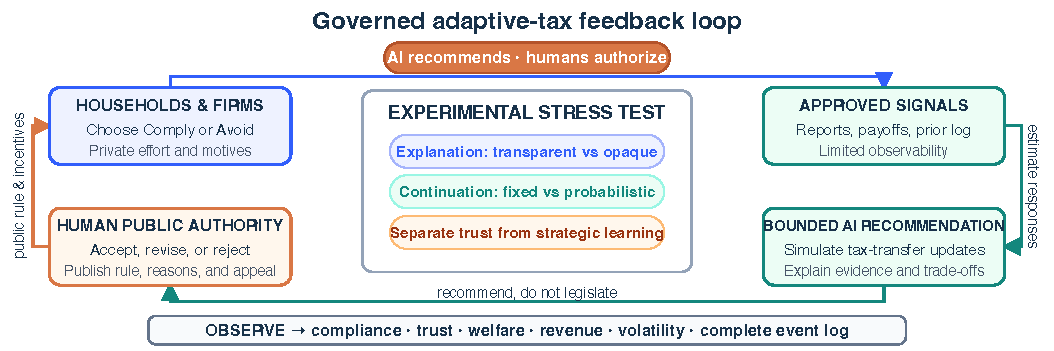
\includegraphics[width=\textwidth]{figures/ps1_teaser.pdf}
\caption{Proposed governed feedback loop for adaptive taxation. Household and firm choices generate approved signals; an auditable system uses them to simulate bounded recommendations; a human authority accepts, revises, or rejects each proposal and publishes the rule, reasons, and appeal route. The stress test varies explanation and continuation incentives to distinguish institutional trust~\cite{kirchler2008} from strategic learning~\cite{suttonbarto2018}. Arrows show the proposed mechanism, not an observed causal effect.}
\Description{A clockwise loop connects households and firms, approved behavioral signals, a bounded AI recommendation, and a human public authority. The center lists experimental comparisons of transparent versus opaque explanation and fixed versus probabilistic continuation. A bottom bar lists compliance, trust, welfare, revenue, volatility, and the event log as outcomes. Every object and label is editable in Draw.io.}
\label{fig:teaser}
\end{teaserfigure}
\maketitle\raggedbottom\coursemeta

\section{Three connected research questions}
Tax policy changes reporting behavior, and those reports inform later policy. This loop combines the efficiency--equity problem in optimal taxation~\cite{mirrlees1971,saez2001,nobel1996} with a new governance risk: opaque learning may undermine legitimacy.

\textbf{Q1---Economics:} Under asymmetric information, when can transparent, bounded policy updates sustain compliance and welfare better than opaque updates?\par
\textbf{Q2---Computation:} Can an auditable finite-state simulator compare those regimes while enforcing bounds and reproducing every transition?\par
\textbf{Q3---Behavior:} Is any cooperation explained by trust in legitimate authority, or only by payoff-based strategic learning?\par
Incentives define the benchmark, computation makes the loop checkable, and behavior determines whether transparency changes choices. Figure~\ref{fig:teaser} joins the three channels.

\section{Answer to Q1: incentives and intellectual lineage}
My hypothesis is that bounded explanations preserve cooperation only when trust or continuation value supplements material payoffs. For eight simultaneous rounds, a taxpayer chooses Comply (C) or Avoid (A), and an authority Transparent (T) or Opaque (O). Model-set payoffs are C/T $=(3,3)$, C/O $=(0,4)$, A/T $=(4,0)$, and A/O $=(1,1)$. Both see the rule, trust score, and prior log, but not private motives. A and O are strictly dominant, making A/O the unique one-shot Nash equilibrium~\cite{nash1950}; C/T is Pareto-superior. Finite repetition with unchanged payoffs does not reverse that benchmark, so persistent C/T requires future incentives, beliefs, or social preferences---not a displayed trust score alone.

\section{Answer to Q2: method and evaluation}
The client-side finite-state game adds payoffs, updates trust by $+10,-15,-10,-10$, clips it to $[0,100]$, and logs every transition. Verified demonstrations produced $24/24$/100 (eight C/T), $7/11$/0 (one C/O then seven A/O), and $23/19$/90 (mixed recovery), where entries are taxpayer payoff/authority payoff/trust. These checks validate code, not behavior. The smallest experiment randomizes explained versus opaque updates with fixed payoffs; a modification varies observability. Colab must reproduce the rules, while Hugging Face provides the interactive interface.

\clearpage\balance
\section{Answer to Q3: behavior and competing explanations}
The slippery-slope mechanism predicts that transparent authority builds trust and voluntary compliance~\cite{kirchler2008}; strategic learning instead predicts cooperation only when future rewards justify it. A preregistered $2\times2$ test can vary explanation and continuation probability, measuring choices, comprehension, legitimacy, and payoffs. An explanation effect surviving payoff and comprehension controls favors trust; disappearance without continuation incentives favors learning. The model would add either trust-dependent utility or belief-dependent continuation value and log them separately. A classroom sample cannot identify population or policy effects. I would reject the trust claim if explanation changes comprehension but not behavior or legitimacy.


\section{Advanced development and future directions}
Mirrlees established how private information constrains tax incentives~\cite{mirrlees1971,nobel1996}; Sutton and Barto's Turing-recognized work established learning from feedback~\cite{acm2024}. The enduring question is how institutions secure fair cooperation without complete surveillance. Today's software can update rapidly and log decisions, but when recommendations remain incentive-compatible, understandable, and legitimate is unresolved. I contribute a bounded-update model, reproducible audit, and test separating trust from continuation incentives.

\begin{table}[h]\caption{From laureate foundations to a new interdisciplinary contribution.}
\begin{tabularx}{\columnwidth}{@{}p{1.6cm}Y@{}}\toprule
\textbf{Horizon}&\textbf{Milestone and evidence}\\\midrule
Foundation&Mirrlees: private-information tax incentives; Sutton--Barto: feedback learning.\\
PS1&Auditable game; three path checks.\\
Next study&Vary explanation and continuation value.\\
Longer term&Add diverse samples, legal rules, and privacy audits.\\
2056&Contestable adaptive institutions supported by field evidence.\\\bottomrule
\end{tabularx}\end{table}

\noindent\textbf{Expected 2056 Nobel Prize and Turing Award contribution statement.}
By 2056, I aspire to be recognized for designing adaptive tax institutions that people can understand and challenge. Building on Mirrlees and Sutton--Barto, I will integrate public economics, auditable computation, and behavioral evidence to determine when learning improves opportunity without sacrificing privacy or legitimacy. Evidence must progress from reproducible pilots to discriminating experiments, cross-jurisdiction validation, and accountable deployment.

\subsection*{Open Science Statement}
\textbf{GitHub:} \GitHubLink\\
\textbf{Google Colab:} \ColabLink\par
Synthetic inputs and client-side code reproduce the three paths. Before submission, add the final commit and verify a clean Colab ``Run all.'' Source-specific licenses remain in their repositories.

\subsection*{Statement of Contribution to the UN's SDGs}
\textbf{Hugging Face:} \DemoLink\\
The open browser game supports \textbf{SDG 4---Quality Education}~\cite{sdg4}: students choose both players' actions, inspect the log, and compare paths to learn repeated games, transparency, and trust. A pre/post prediction task could assess learning; improvement remains untested.

\subsection*{Submission milestones}
First draft: September 13, 2026, 11:00 P.M. Beijing time (UTC+8). Class review: September 14. Proposed: rebuttal September 16 and revised submission September 20, both at 11:00 P.M. Update Appendix~\ref{app:abstract} with each reflection and revision.

\clearpage\nobalance
\section*{Author Notes}
\subsection*{Acknowledgements}
I thank Prof. Luyao Zhang, Program Chair, and Prof. Ken Rogerson, Program Discussant, of the \emph{2056 Nobel and Turing Laureate Program Launch Workshop}, held at Duke Kunshan University on September 7, 2026. I also thank Gihun and Zimu, my teammates in session E, and the rest of the COMSCI/ECON 206 Autumn 2026 Session 1 class for their questions and discussion. Lin Zhang's earlier feedback helped me replace the claim of an autonomous ``self-evolving AI tax system'' with a human-authorized, bounded, and contestable institution. I am responsible for the proposal and remaining errors.
\subsection*{Individual contribution}
I selected the adaptive-tax research question, designed the taxpayer--authority game and its payoff and trust rules, supplied the field photographs, tested all three eight-round paths in the deployed Space, and made the final decisions about claims and limitations. I adapted the course Overleaf structure and Figure~\ref{fig:teaser} to this project. The course template and cited open-source tools are credited separately and do not imply coauthorship.

\bibliographystyle{ACM-Reference-Format}\bibliography{references}
\appendix
\section{Technical details and reproducibility}
The game state is $(r,t,p_T,p_A,L)$: round, trust, taxpayer payoff, authority payoff, and event log. It begins at $(1,50,0,0,[])$. Each action pair selects a payoff and trust increment from Table~\ref{tab:rules}; the update is $t'=\min\{100,\max\{0,t+\Delta t\}\}$. There is no random seed because the current browser artifact is deterministic. Reset restores the initial state.

\begin{table}[h]
\caption{Programmed stage-game and trust rules.}
\label{tab:rules}
\centering
\begin{tabular}{@{}llcc@{}}\toprule
Taxpayer & Authority & Payoff $(T,A)$ & $\Delta$ trust\\\midrule
Comply & Transparent & $(3,3)$ & $+10$\\
Comply & Opaque & $(0,4)$ & $-15$\\
Avoid & Transparent & $(4,0)$ & $-10$\\
Avoid & Opaque & $(1,1)$ & $-10$\\\bottomrule
\end{tabular}
\end{table}

The deployed Static Space was accessed and personally tested on September 6, 2026. Eight C/T rounds returned $24/24$, trust 100; C/O followed by seven A/O returned $7/11$, trust 0; and C/T, C/T, A/T, A/O, then four C/T returned $23/19$, trust 90. Each run produced eight log entries; the first two also checked the upper and lower trust bounds. The implementation uses client-side HTML, CSS, and JavaScript with no backend, database, API key, paid service, or personal-data collection. The Python companion independently reproduces the payoff, trust-bound, event-log, invalid-input, and one-shot-equilibrium checks using only the standard library. It does not establish calibrated tax payoffs, legal accuracy, real compliance behavior, or population effects. After the code is pushed to GitHub, the Colab notebook will be run from a clean session and the submitted code commit recorded in the Open Science Statement.
\subsection{AI-use disclosure}
I used OpenAI Codex in the Codex desktop interface on September 13, 2026, after developing the research direction in my first two intellectual statements. It helped organize and edit the proposal, adapt the LaTeX template and editable teaser, check the payoff arithmetic, and format references and appendices. I retained the human-authority boundary, the trust-versus-incentives distinction, and explicit limits on synthetic evidence; I rejected any claim that the game demonstrates real taxpayer behavior. I will review the final Overleaf rendering, verify the URLs and citations, and remain responsible for every claim and computation.

\section{Cumulative Intellectual Development}
This proposal develops my Intellectual Statements I and II through the \emph{2056 Nobel and Turing Laureate Program Launch Workshop}, held on September 7, 2026 at Duke Kunshan University, IB 2050. Program Chair: Prof. Luyao Zhang. Program Discussant: Prof. Ken Rogerson. My session: Session E. My role: Economist. My teammates: Gihun and Zimu. I acknowledge their contributions and the rest of the class's questions and discussion.

My first statement proposed a ``self-evolving AI tax system.'' Lin Zhang's August 30 feedback and my subsequent reflection exposed the risk that this language assigned legislative authority to AI. Intellectual Statement II therefore made public officials the decision makers and required bounded, explained recommendations. The September 4 Tencent and museum observations then sharpened explanation into an interface requirement: feedback should be familiar, while rules, evidence, limits, and trade-offs should remain visible. Finally, the Week 2 implementation showed that a trust counter can be computed reproducibly but does not itself explain behavior. This proposal consequently separates the Nash benchmark, trust-based utility, and continuation incentives, and proposes a test that can discriminate among them. During the September 7 workshop, a classmate asked whether the trust score actually changed players' incentives or merely displayed the history of play. This question led me to treat trust as a mechanism to be tested rather than an assumed explanation and to vary continuation incentives separately in the proposed experiment.
Appendix~\ref{app:abstract} records the eight-part structured abstract in the cumulative reflection format and connects the 2056 contribution statement to the foundation, current-era boundary, and interdisciplinary milestones.

\section{Field and open-source inspiration}
I attended the \emph{Joint Interdisciplinary Field Trip---Technology, Computation, Culture \& Society in Action} on September 4, 2026, visiting \textbf{Tencent Shanghai Office} and \textbf{Shanghai Science and Technology Museum}. The observations below are first-hand; the design lessons are my interpretations, not causal evidence.

\begin{figure*}[ht]
\centering
\begin{minipage}[t]{0.48\textwidth}\centering
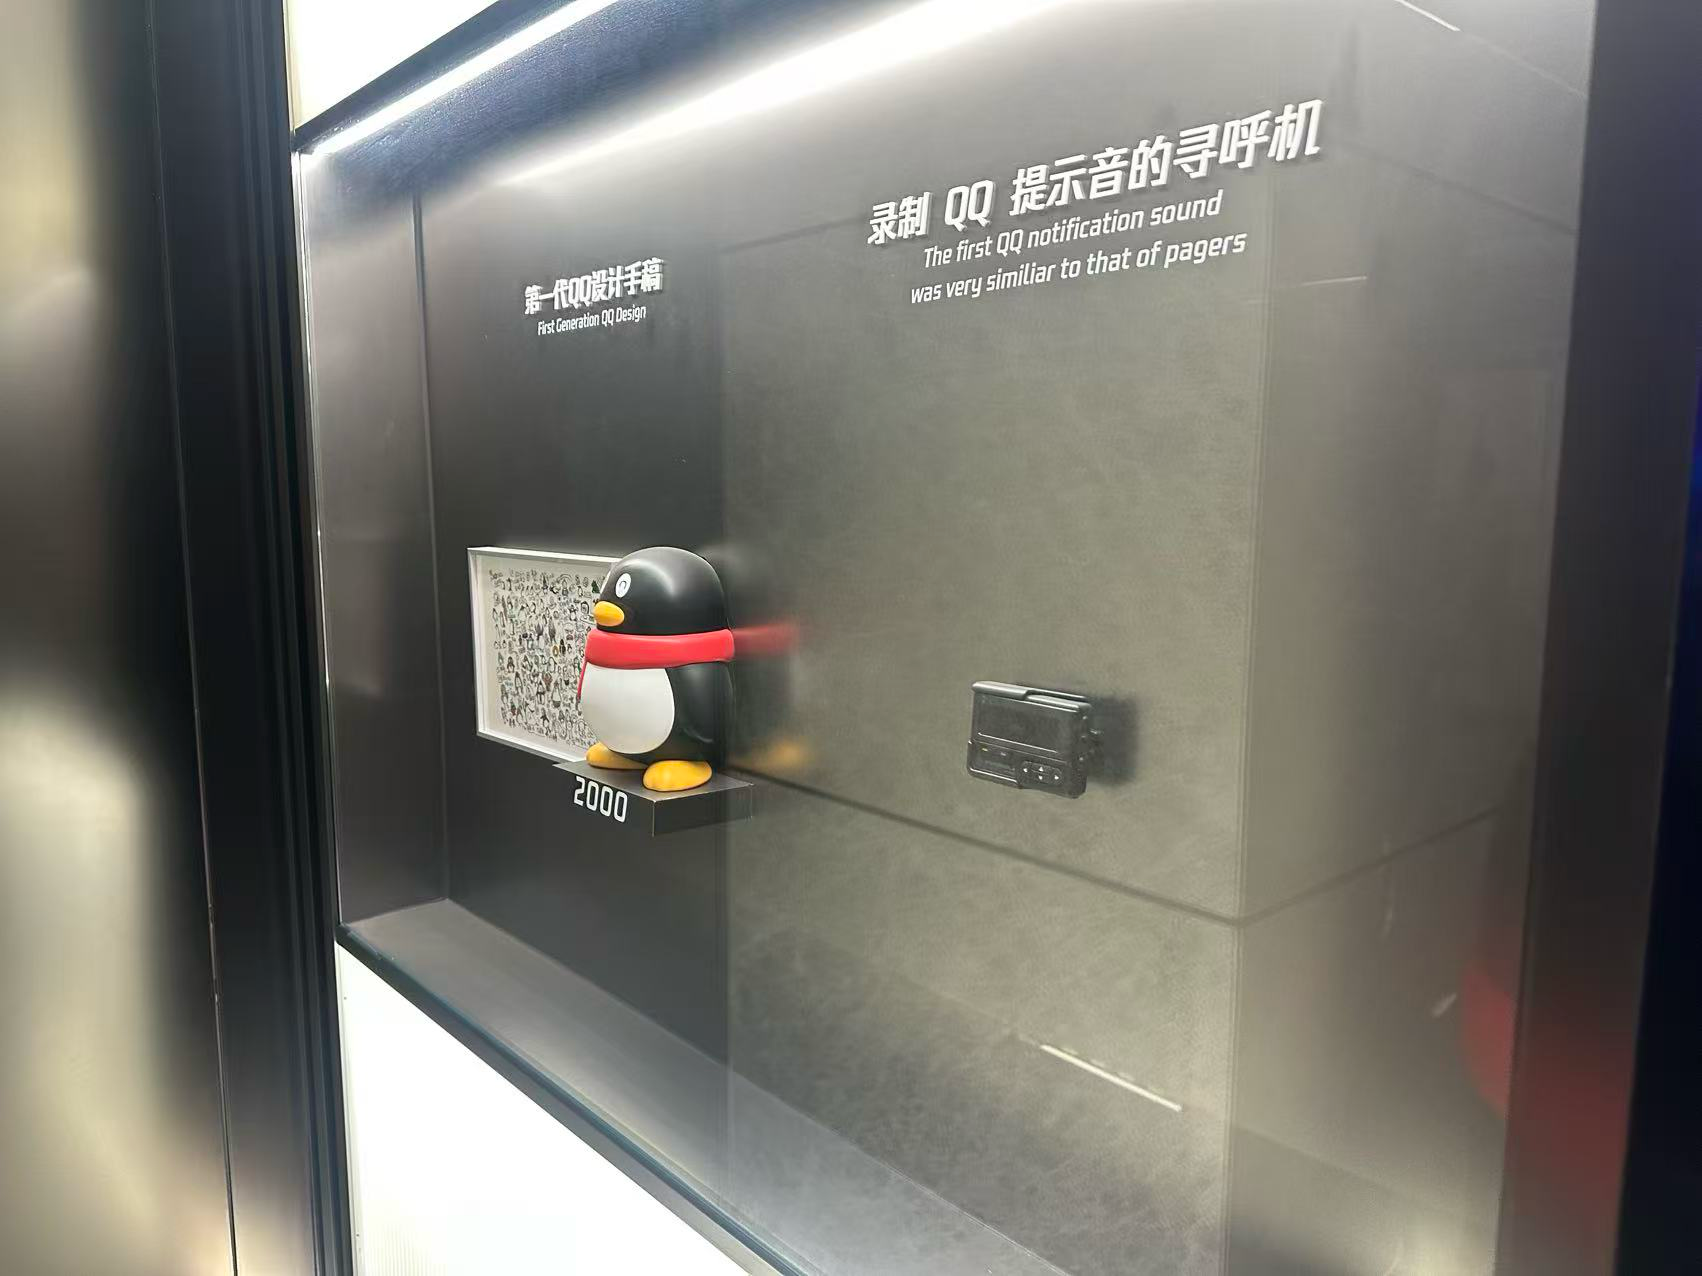
\includegraphics[width=\linewidth,height=4.2cm,keepaspectratio]{figures/tencent_qq_exhibit.png}
\small\textbf{(a) Tencent Shanghai Office, September 4, 2026.} Photograph by the author. The exhibit presented the first-generation QQ design and its pager-like notification sound. I interpret the familiar cue as inspiration for explanations that help users recognize a policy update.
\end{minipage}\hfill
\begin{minipage}[t]{0.48\textwidth}\centering
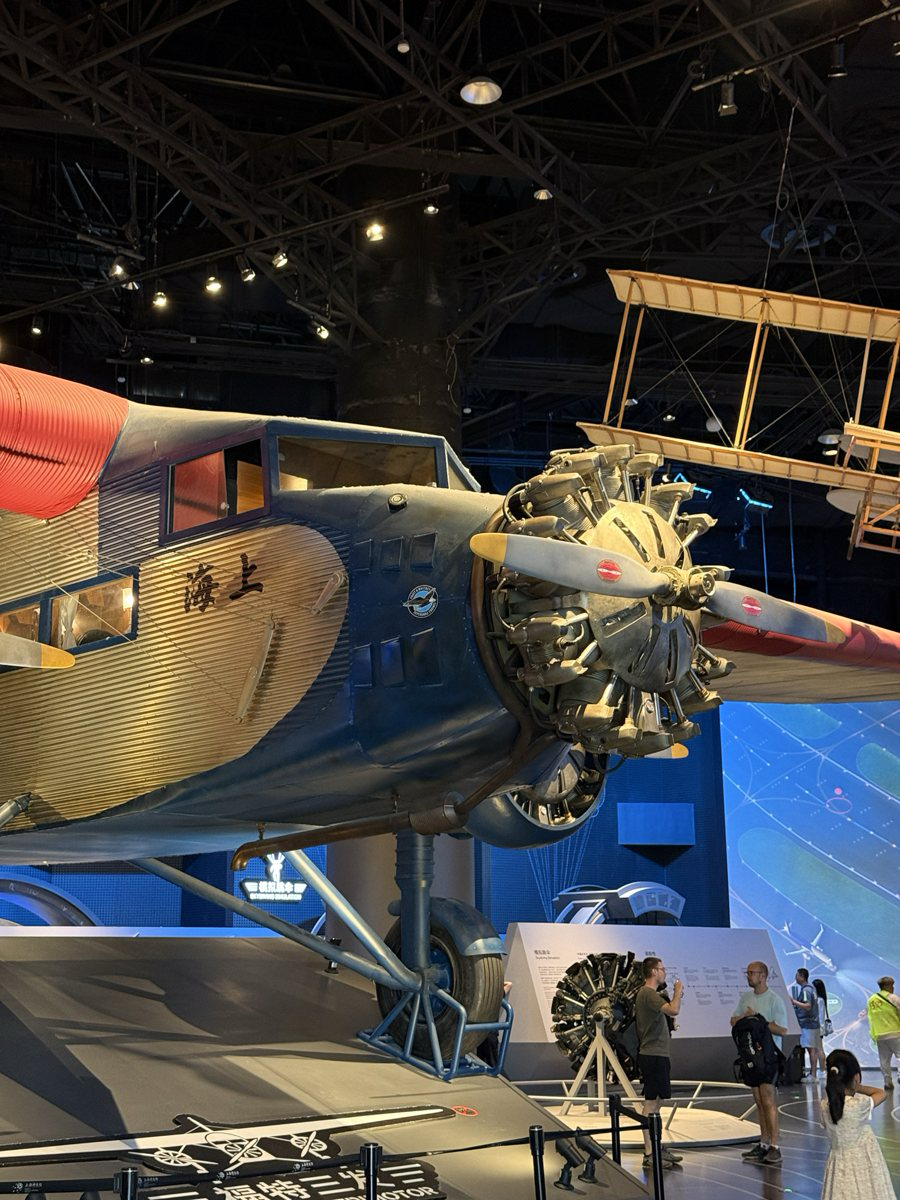
\includegraphics[width=\linewidth,height=4.2cm,keepaspectratio]{figures/shanghai_museum_aircraft.png}
\small\textbf{(b) Shanghai Science and Technology Museum, September 4, 2026.} Photograph by the author. An early aircraft display left its engine and supports visible. I interpret this as inspiration for exposing a recommendation's rule, evidence, limits, and trade-off.
\end{minipage}
\caption{Field evidence retained from Intellectual Statement II. The photographs document exhibits; the proposed interface implications remain hypotheses.}
\Description{Left: a first-generation QQ penguin exhibit beside a pager and explanatory text. Right: an early aircraft displayed indoors with its radial engine and structural supports visible.}
\label{fig:field}
\end{figure*}

EconML 0.16.0 can estimate heterogeneous effects offline, but it cannot remove confounding from poor data~\cite{econml}. OpenFisca Core 44.7.0 can turn public tax rules into inspectable code, but it requires maintained jurisdiction-specific packages and does not predict behavior~\cite{openfisca}. Together they suggest a division of labor: estimate responses cautiously, execute legal rules transparently, and keep policy authority with humans. Potential private-sector value is testing whether automated messages are understood across user groups; public-sector value is showing how a tax or benefit result follows from an inspectable rule.

\section{Review response and revision record}
This is the September 13 v1 draft. Peer reviews, author response, reviewer follow-up, and v2 are pending. Preserve this source and compiled PDF before revision. After the September 14 review, record (1) strengths retained, (2) constructive concerns and changed locations, and (3) questions answered or deferred, together with verification results. Do not overwrite the v1 record.

\clearpage\onecolumn
\section{Structured abstract and cumulative proposal map}\label{app:abstract}
The first seven rows summarize the current research proposal; the final row records feedback and the resulting intellectual revision.
\par\medskip
\begin{table}[H]
\caption{Appendix E structured abstract and cumulative proposal map.}
\label{tab:abstract-map}
\renewcommand{\arraystretch}{1.18}
\begin{tabularx}{\textwidth}{@{}p{0.27\textwidth}Y@{}}
\toprule
\textbf{Proposal element} & \textbf{Current statement / change} \\
\midrule
Background & Adaptive tax recommendations create a feedback loop: behavior changes the data used for later policy. Mirrlees established incentive constraints under private information; the unresolved issue is legitimate adaptation. \\
Motivation and application & Faster policy software may improve opportunity but can also invite gaming, surveillance, or distrust. Taxpayers, officials, and beneficiaries need updates that are effective and contestable. \\
Three connected questions & Economics: when do bounded transparent updates improve compliance and welfare? Computation: can an auditable simulator test them? Behavior: does trust or strategic learning explain cooperation? Integration is required because each answer changes the others. \\
Method and model assumptions & An eight-round taxpayer--authority game compares Comply/Avoid and Transparent/Opaque under public rules but private motives. A deterministic state machine records payoffs, bounded trust, and every transition; the next study randomizes transparency and continuation value. \\
Results or expected results & Three programmed paths reproduce $24/24$/100, $7/11$/0, and $23/19$/90 (payoffs/trust). These are implementation checks. I expect transparent bounded feedback to support cooperation; no behavioral effect would challenge the claim. \\
Intellectual merits & The proposal connects incentive-compatible taxation, auditable feedback algorithms, and a discriminating behavioral test, while showing why a computed trust score is not behavioral evidence. \\
Practical impacts & Firms could test message comprehension; agencies could expose executable benefit rules. The open browser game supports SDG 4 instruction; a pre/post prediction task would test learning value. \\
Feedback received and revision made & August 30 feedback from Lin Zhang and later reflection changed an autonomous ``self-evolving'' system into human-authorized, bounded recommendations. September 4 field evidence added visible explanations. During the September 7 workshop, a classmate asked whether the trust score changed players’ incentives or merely summarized the history of play. I therefore separated trust-based utility from continuation incentives and added a \(2 \times 2\) test varying explanation transparency and continuation probability. Peer review is pending. \\
\bottomrule
\end{tabularx}
\end{table}

\end{document}
